% =====================================================================
% Fig. 5 - Sparse-Period Kernel (SPK), FEATHer module [4].
%
% Direct R6 #4(c) defense:
%   (1) Vector TikZ render -> no blur at column width.
%   (2) The on-figure formula matches the main-text Eq. (10) exactly:
%       \widehat{Y}_d(p, :) = H'_d(p, :) W,
%       where each phase row uses the same shared W.
%
% Pipeline:
%   H -> [DWConv pre-mix]       ... H' \in R^{B x L x D}
%     -> [period reshape: P phases x n cols]
%     -> [shared linear W : n -> m]
%     -> [P phases x m cols]
%     -> [interleave back -> 1D]   ... \widehat{Y} \in R^{B x H x D}
%
% n = L/P (periods per phase),  m = H/P (forecast period count).
% =====================================================================
\documentclass[tikz, border=8pt]{standalone}

\usepackage{amsmath, amssymb}
\usepackage{tikz}
\usetikzlibrary{arrows.meta, positioning, calc, decorations.pathreplacing}

\definecolor{pointC}{HTML}{6B7280}
\definecolor{highC}{HTML}{DC2626}
\definecolor{midC}{HTML}{F59E0B}
\definecolor{lowC}{HTML}{2563EB}

\begin{document}

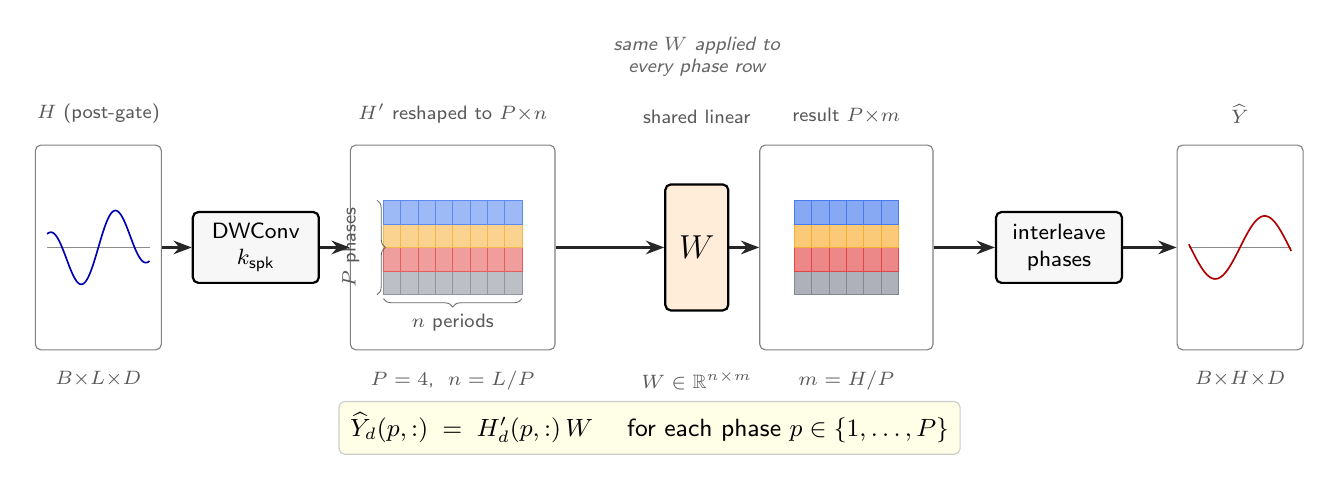
\begin{tikzpicture}[
    font=\sffamily\small,
    >=Stealth,
    op/.style={
        draw, thick,
        rounded corners=2pt,
        fill=gray!6,
        minimum width=1.6cm,
        minimum height=0.9cm,
        align=center,
        font=\sffamily\footnotesize,
        inner sep=2pt
    },
    wbox/.style={
        draw, thick,
        rounded corners=2pt,
        fill=orange!10,
        minimum width=0.8cm,
        minimum height=1.6cm,
        align=center,
        font=\sffamily\footnotesize\bfseries
    },
    panel/.style={
        draw=black!50, line width=0.4pt,
        rounded corners=2pt,
        fill=white
    },
    flow/.style={->, thick, draw=black!85},
    caption/.style={font=\sffamily\scriptsize, text=black!65},
    axis/.style={draw=black!45, line width=0.3pt}
]

% =====================================================================
% Geometry — left to right pipeline
% =====================================================================
\def\xH{0}          % input H (1D time series)
\def\xPre{2.0}      % DWConv pre-mix
\def\xGridIn{4.5}   % P x n grid (after reshape)
\def\xW{7.6}        % shared linear W
\def\xGridOut{9.5}  % P x m grid
\def\xInter{12.2}   % interleave op
\def\xYhat{14.5}    % output forecast

% =====================================================================
% Stage 1: Input H (1D time series after gating fusion)
% =====================================================================
\node[panel, minimum width=1.6cm, minimum height=2.6cm] (HBOX) at (\xH, 0) {};
\node[caption, anchor=south] at (\xH, 1.45) {$H$ (post-gate)};
\node[caption, anchor=north] at (\xH, -1.45) {$B{\times}L{\times}D$};
\begin{scope}[shift={(\xH, 0)}]
    \draw[axis] (-0.65, 0) -- (0.65, 0);
    \draw[blue!70!black, line width=0.6pt, smooth, samples=80, domain=-0.65:0.65]
        plot (\x, {0.35*sin(8*\x r) + 0.18*sin(3.5*\x r)});
\end{scope}

% =====================================================================
% Stage 2: DWConv pre-mix
% =====================================================================
\node[op] (PRE) at (\xPre, 0) {DWConv\\$k_\text{spk}$};

% =====================================================================
% Stage 3: P x n grid (after period reshape)
%   P = 4 phases (rows), n = 8 periods (cols)
% =====================================================================
\node[panel, minimum width=2.6cm, minimum height=2.6cm] (GIN) at (\xGridIn, 0) {};
\node[caption, anchor=south] at (\xGridIn, 1.45) {$H'$ reshaped to $P{\times}n$};
\node[caption, anchor=north] at (\xGridIn, -1.45) {$P=4$,\ \ $n = L/P$};
\begin{scope}[shift={(\xGridIn, 0)}]
    \def\cw{0.22}
    \def\ch{0.30}
    \def\gxL{-0.88}
    \def\gyB{-0.60}
    % Row colors = phase (R2 #2 palette: gray/red/amber/blue)
    \foreach \r/\col in {0/pointC, 1/highC, 2/midC, 3/lowC} {
        \foreach \c in {0,1,...,7} {
            \pgfmathsetmacro{\cx}{\gxL + \c*\cw}
            \pgfmathsetmacro{\cy}{\gyB + \r*\ch}
            \fill[\col!45] (\cx, \cy) rectangle (\cx + \cw, \cy + \ch);
            \draw[\col!75, line width=0.2pt] (\cx, \cy) rectangle (\cx + \cw, \cy + \ch);
        }
    }
    % left brace: P phases
    \draw[decorate, decoration={brace, amplitude=3pt}, draw=black!60, line width=0.3pt]
        (\gxL - 0.08, \gyB + 4*\ch) -- (\gxL - 0.08, \gyB);
    \node[caption, rotate=90, anchor=south] at (\gxL - 0.18, \gyB + 2*\ch) {$P$ phases};
    % bottom brace: n cols
    \draw[decorate, decoration={brace, mirror, amplitude=3pt}, draw=black!60, line width=0.3pt]
        (\gxL, \gyB - 0.05) -- (\gxL + 8*\cw, \gyB - 0.05);
    \node[caption, anchor=north] at (\gxL + 4*\cw, \gyB - 0.12) {$n$ periods};
\end{scope}

% =====================================================================
% Stage 4: shared linear W (n -> m)
% =====================================================================
\node[wbox, font=\sffamily\large\bfseries, fill=orange!15] (WMAT) at (\xW, 0) {$W$};
\node[caption, anchor=south] at (\xW, 1.45) {shared linear};
\node[caption, anchor=north] at (\xW, -1.45) {$W \in \mathbb{R}^{n \times m}$};

% =====================================================================
% Stage 5: P x m grid (after linear projection)
% =====================================================================
\node[panel, minimum width=2.2cm, minimum height=2.6cm] (GOUT) at (\xGridOut, 0) {};
\node[caption, anchor=south] at (\xGridOut, 1.45) {result $P{\times}m$};
\node[caption, anchor=north] at (\xGridOut, -1.45) {$m = H/P$};
\begin{scope}[shift={(\xGridOut, 0)}]
    \def\cw{0.22}
    \def\ch{0.30}
    \def\gxL{-0.66}
    \def\gyB{-0.60}
    \foreach \r/\col in {0/pointC, 1/highC, 2/midC, 3/lowC} {
        \foreach \c in {0,1,...,5} {
            \pgfmathsetmacro{\cx}{\gxL + \c*\cw}
            \pgfmathsetmacro{\cy}{\gyB + \r*\ch}
            \fill[\col!55] (\cx, \cy) rectangle (\cx + \cw, \cy + \ch);
            \draw[\col!85, line width=0.2pt] (\cx, \cy) rectangle (\cx + \cw, \cy + \ch);
        }
    }
\end{scope}

% =====================================================================
% Stage 6: Interleave-phases operator
% =====================================================================
\node[op] (INT) at (\xInter, 0) {interleave\\phases};

% =====================================================================
% Stage 7: Forecast Yhat (1D)
% =====================================================================
\node[panel, minimum width=1.6cm, minimum height=2.6cm] (YHAT) at (\xYhat, 0) {};
\node[caption, anchor=south] at (\xYhat, 1.45) {$\widehat{Y}$};
\node[caption, anchor=north] at (\xYhat, -1.45) {$B{\times}H{\times}D$};
\begin{scope}[shift={(\xYhat, 0)}]
    \draw[axis] (-0.65, 0) -- (0.65, 0);
    \draw[red!70!black, line width=0.6pt, smooth, samples=80, domain=-0.65:0.65]
        plot (\x, {0.4*sin(5*\x r + 0.4)});
\end{scope}

% =====================================================================
% Flow arrows
% =====================================================================
\draw[flow] (HBOX.east)   -- (PRE.west);
\draw[flow] (PRE.east)    -- (GIN.west);
\draw[flow] (GIN.east)    -- (WMAT.west);
\draw[flow] (WMAT.east)   -- (GOUT.west);
\draw[flow] (GOUT.east)   -- (INT.west);
\draw[flow] (INT.east)    -- (YHAT.west);

% =====================================================================
% Central formula (matching main text Eq.(10) exactly)
% =====================================================================
\node[font=\sffamily\small, anchor=north, fill=yellow!10, draw=black!20,
      rounded corners=2pt, inner sep=4pt]
    at ({(\xGridIn + \xGridOut)/2}, -1.95)
    {$\widehat{Y}_d(p, :) \;=\; H'_d(p, :)\, W$
     \quad for each phase $p \in \{1, \ldots, P\}$};

% =====================================================================
% Weight-sharing annotation: arrow from W down to formula
% =====================================================================
\node[font=\sffamily\scriptsize\itshape, text=black!60, anchor=south, align=center]
    at (\xW, 2.05)
    {same $W$ applied to\\every phase row};

\end{tikzpicture}

\end{document}
